\subsection{Integracja konturów modelem integrate-and-fire}
\label{integracjaSPIKE}

\begin{figure}[ht]
	\centering
	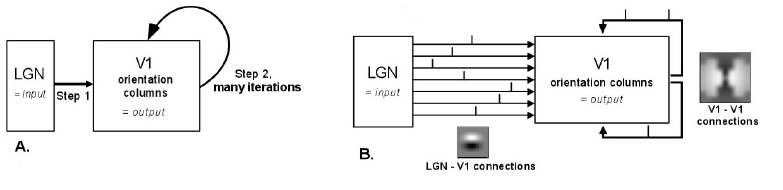
\includegraphics[width=1\textwidth]{images/spike_model.png}
	\caption{Przedstawienie porównań modeli integracji konturów w pierwszorzędowej korze wzrokowej \cite{Vanrullen2001}.}
	\label{fig:spike_model}
\end{figure}

%\begin{figure}[ht]
%	\centering
%	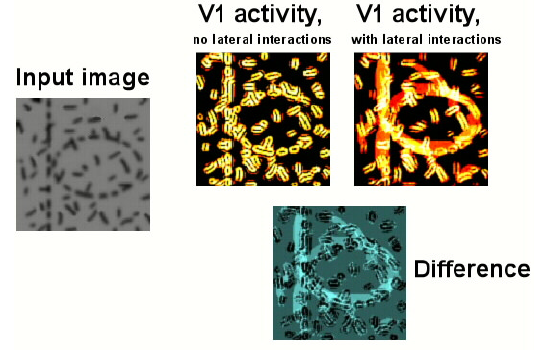
\includegraphics[width=0.65\textwidth]{images/spike_model_out_1.png}
%	\caption{ \cite{Vanrullen2001}.}
%	\label{fig:spike_model_out_1}
%\end{figure}

%\begin{figure}[ht]
%	\centering
%	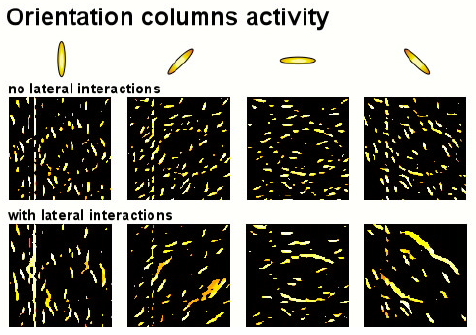
\includegraphics[width=0.65\textwidth]{images/spike_model_out_2.png}
%	\caption{ \cite{Vanrullen2001}.}
%	\label{fig:spike_model_out_2}
%\end{figure}

\begin{figure}[ht]
	\centering
	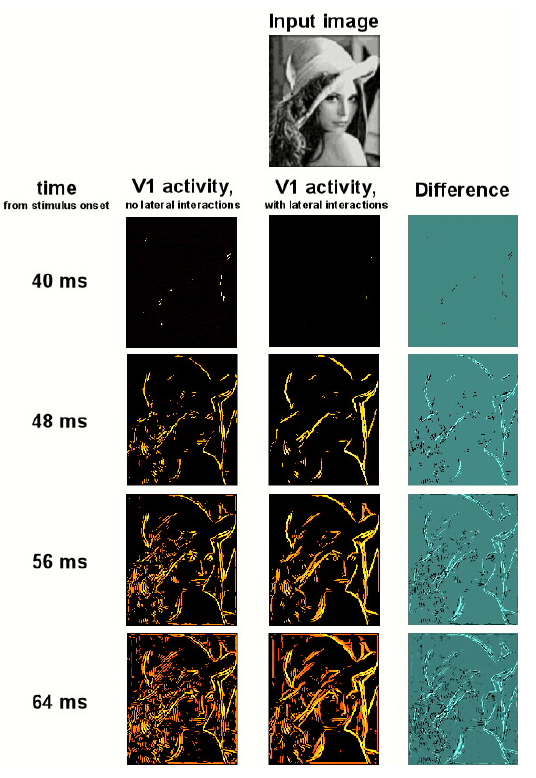
\includegraphics[width=0.65\textwidth]{images/spike_model_results.png}
	\caption{Porównanie wyników otrzymywanych z modelu ,,integrate-and-fire'' ze sprzężeniem i bez \cite{Vanrullen2001}.}
	\label{fig:spike_model_results}
\end{figure}
%spike - 10003
%TODO - przeformułowanie początku

Autorzy pracy \cite{Vanrullen2001} zauważyli pewien mankament zwłaszcza wydajnościowy w modelu przedstawionym choćby w poprzedniej części -- \ref{integracjaLi}. Podstawową jego cechą były dziesiątki połączeń miedzy neuronami z hiperkolumn, przez co przeliczanie się całości trwało jakiś czas. Na podobnej zasadzie autorzy przytaczają też inne publikacje.\\

Głównym argumentem -- który zdaniem autora tego dokumentu jest śmieszny -- który stał za wnioskiem, że wyliczone modele są złe, był czas ich działania. Porównując je bowiem z błyskawicznym\footnote{W publikacji jest to określone angielskim słowem rapid.} przetwarzaniem obrazów w korze wzrokowej człowieka, bądź małpy, muszą one być w sprzeczności z całą biologią, która za tym stoi. Nie podejmowano jednak argumentu, że w mózgu absolutnie wszystko jest ,,przeliczane'' równolegle i nie ma w nim miejsca na iteracje znane z komputerowych implementacji sieci neuronowych. Nie mniej jednak proponuje się w tej pracy specyficzne podejście bazujące na modelu ,,sumuj i strzelaj\footnote{Tłumaczenie z języka angielskiego frazy integrate-and-fire, którą można nazwać inaczej modelem Lapicque'a\cite{Lapicque}.}''. Zaproponowany model przedstawia rysunek \ref{fig:spike_model}B. Autorzy porównują go do proponowanych w innych pracach iteracyjnych podejść, które przedstawione są na rysunku \ref{fig:spike_model}A. Na pierwszy rzut oka nie widać specjalnie różnic, podstawowa wynikająca z zastosowania podejścia Lapicque'a jest jednak -- zdaniem autorów -- kluczowa.\\

W modelu widać wyraźnie sprzężenie zwrotne i mimo, że są one krytykowane w cytowanych wcześniej pracach, to autorzy podkreślają, że to nie jest problem samych sprzężeń. Chodzi, raczej o to, że w klasycznych modelach sprzężenie zwrotne działa po przeliczeniu się wszystkich neuronów, tutaj jednak, przez wzgląd na obserwacje kory wzrokowej kota sprzężenie zwrotne cały czas ma wpływ na neurony warstwy V1. Całą implementację upraszcza dodatkowo fakt, że przez połączenia prowadzone są jedynie pewne piki, a same neurony zliczają je i na tej podstawie określają swój stan. Nie potrzeba tutaj przesyłania ciągłych sygnałów.\\

Rysunek \ref{fig:spike_model_results} przedstawia otrzymywane w ten sposób rezultaty, które zgodnie z poprzednim akapitem zostały sobie przeciwstawione. Po lewej stronie rezultaty prezentują wyjście z modelu, w którym połączeń między elementami pierwszorzędowej kory wzrokowej nie ma, środkowe obrazy przedstawiają te same wyniki modelu, z różnicą na występowanie połączeń między elementami V1. Prawa kolumna pokazuje różnice między opisanymi rezultatami. Tak jak i w dziesiątkach książek poświęconych grafice komputerowej i tutaj obrazem do testowania była Lena. Podstawowym parametrem modelu jest czas, jaki się poświęca przeliczeniom samego modelu. Otrzymywane rezultaty przedstawiają przede wszystkim zalety korzystania z połączeń między elementami obszaru V1 jak i samego pomysłu na realizację integracji konturów w korze wzrokowej.\\

